\documentclass[12pt, twoside]{article}
\usepackage[letterpaper, margin=1in, headsep=0.5in]{geometry}
\usepackage[english]{babel}
\usepackage[utf8]{inputenc}
\usepackage{amsmath}
\usepackage{amsfonts}
\usepackage{amssymb}
\usepackage{tikz}
\usetikzlibrary{quotes, angles}
\usepackage{graphicx}
\usepackage{enumitem}
\usepackage{multicol}

\newif\ifmeta
\metatrue %print standards and topics tags

\title{Regents Geometry}
\author{Chris Huson}
\date{September 2020}

\usepackage{fancyhdr}
\pagestyle{fancy}
\fancyhf{}
\renewcommand{\headrulewidth}{0pt} % disable the underline of the header
\raggedbottom


\fancyhead[LE]{\thepage}
\fancyhead[RO]{\thepage \\ Name: \hspace{4cm} \,\\}
\fancyhead[L]{BECA / Dr. Huson / Geometry 05-Transformations\\* pset ID: 65}

\begin{document}

\subsubsection*{5-7DNQ-Regents-dilation}
\begin{enumerate}
\item A dilation centered at the origin maps the segment $\overline{CD}$ onto $\overline{C'D'}$. The coordinates of the endpoints of these segments are $C(2,2)$, $D(4,-2)$, $C'(5,5)$, and $D'(10,-5)$. Plot the two line segments on the set of axes below and find the scale factor of the dilation.
  \begin{flushright}
    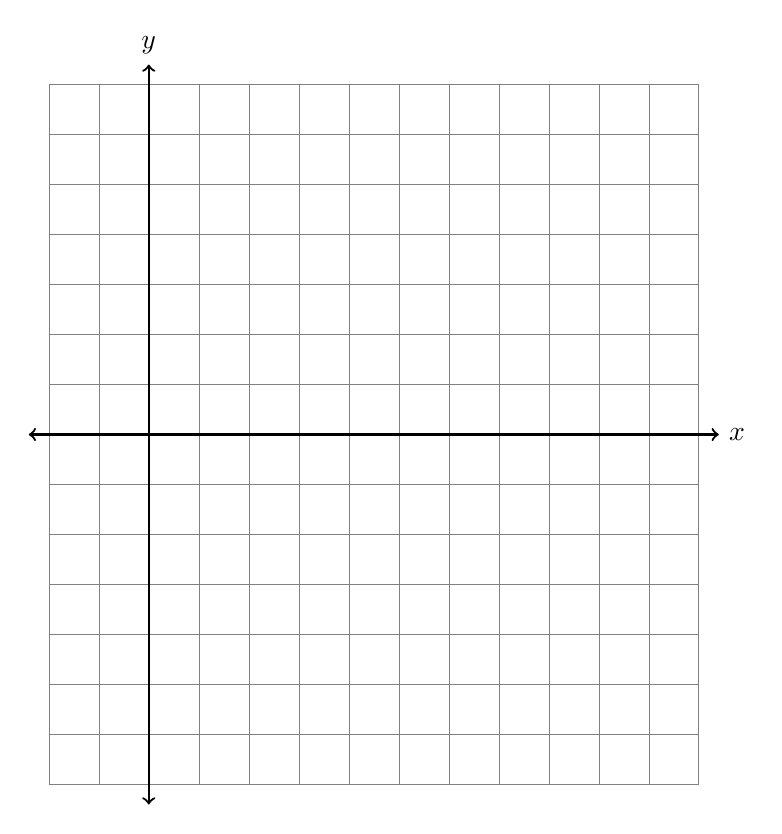
\begin{tikzpicture}[scale=.635]
      \draw [help lines] (-2,-7) grid (11,7);
      \draw [thick, <->] (-2.4,0) -- (11.4,0) node [right] {$x$};
      \draw [thick, <->] (0,-7.4)--(0,7.4) node [above] {$y$};
    \end{tikzpicture}
  \end{flushright}


\item In the diagram below of $\triangle ABC$, $D$ is a point on $\overline{BA}$, $E$ is a point on $\overline{BC}$, and $\overline{DE}$ is drawn. \\*[2pt] 
 If $BD=4$, $BA=10$, and $BE=6$, what is the length of $\overline{EC}$ so that $\overline{AC} \parallel \overline{DE}$?
 
 \begin{flushright}
     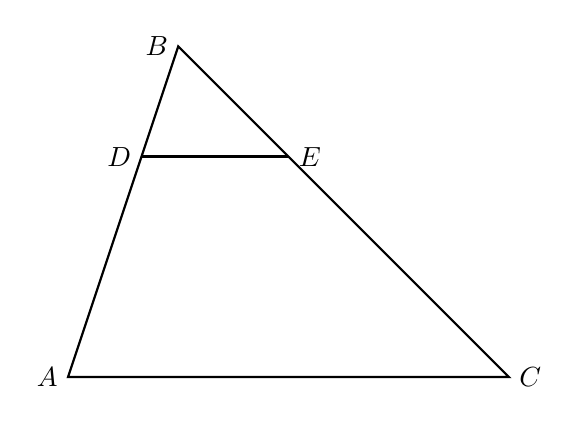
\begin{tikzpicture}[scale=0.7]
       \draw [thick]
       (0,0)node[left]{$A$}--
       (8,0)node[right]{$C$}--
       (2,6)node[left]{$B$}--cycle;
       \draw [thick]
       (4/3,4)node[left]{$D$}--
       (4,4)node[right]{$E$};
     \end{tikzpicture}
   \end{flushright}

\newpage
\subsubsection*{Early finishers}

\item The circle $O$ is shown below with diameter $\overline{AOC}$ and radius $\overline{BO}$. Given that the central angle $m\angle COB=126^\circ$. Find the measure of angle $A$, that is, $m\angle BAO$.
\begin{flushright}
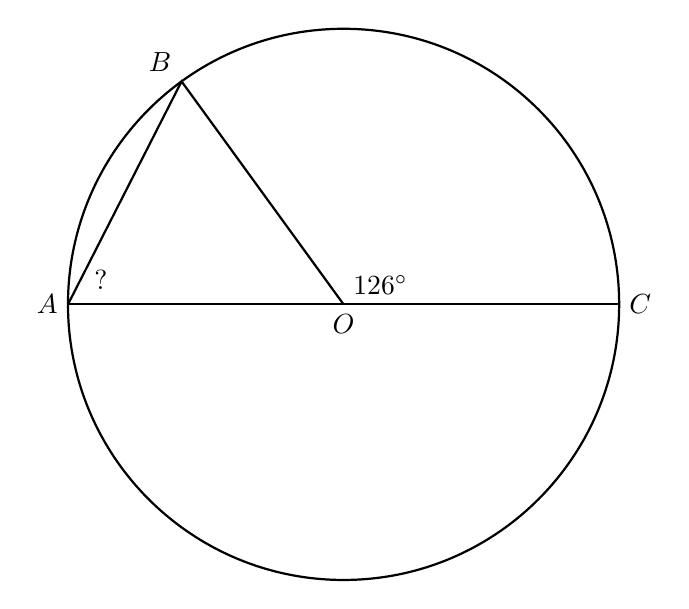
\begin{tikzpicture}[scale=0.7]
  \draw [thick] (0,0) circle [radius=5];
  \draw [-, thick] (-5,0) node[left]{$A$}--
  (0,0) node[below]{$O$}--
  (5,0) node[right]{$C$};
  \draw [-, thick] (0,0)--(126:5) node[above left]{$B$}--(-5,0);
  \node at (0, 0)[above right]{$126^\circ$};
  \node at (-4.7, 0.1)[above right]{?};
\end{tikzpicture}
\end{flushright} %\vspace{2cm}

\item A special shield is cut from gold foil having a shape as shown with lengths marked in inches. (the drawing is not to scale, but the corners are square)
  \begin{enumerate}
    \item Find the area of the figure.
      \begin{flushright}
      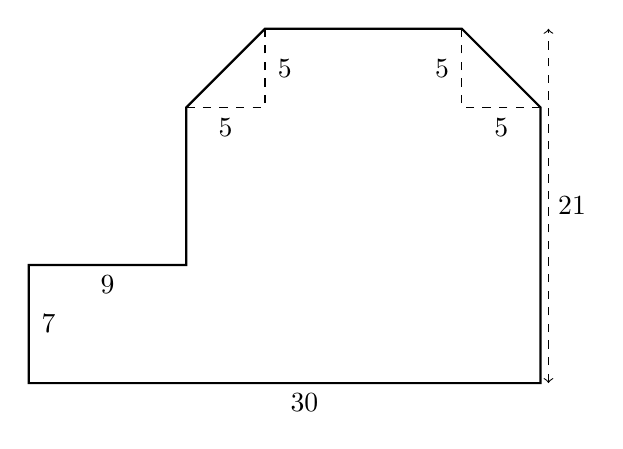
\begin{tikzpicture}[scale=0.5]
        \draw [-, thick] (0,0)--(13,0)--(13,7)--(11,9)--
        (6,9)--(4,7)--(4,3)--(0,3)--cycle;
        \draw [dashed] (4,7)--(6,7)--(6,9);
        \draw [dashed] (13,7)--(11,7)--(11,9);
        \draw [<->, dashed] (13.2,0)--(13.2,9);
        \node at (6.5, 8){5};
        \node at (5, 6.5){5};
        \node at (0.5, 1.5){7};
        \node at (2, 2.5){9};
        \node at (10.5, 8){5};
        \node at (12, 6.5){5};
        \node at (7, -0.5){30};
        \node at (13.8, 4.5){21};
        %\node at (13.5, 8){2};
      \end{tikzpicture}
      \end{flushright} \vspace{2cm}
    \item Spicy: The foil costs \$1250 per square foot. Find the materials cost of the part.
  \end{enumerate}

\end{enumerate}
\end{document}